\documentclass{article}
\usepackage{tikz}
%\usetikzlibrary{trees}

\begin{document}
	
	\begin{center}
		\tikzstyle{level 1}=[level distance=4cm, sibling distance=6cm]
		\tikzstyle{level 2}=[level distance=4cm, sibling distance=3cm]
		
		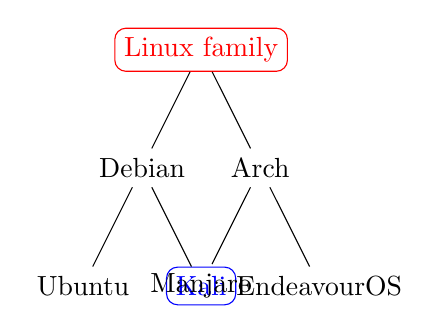
\begin{tikzpicture}[grow=down]
			\node[rounded corners ,draw, red] {Linux family}
			child {
				node{Debian}
				child {
					node {Ubuntu}
					}
				child {
					node[rounded corners ,draw, blue]  {Kali}
					}
			}
			child {
				node {Arch}
				child {
					node {Manjaro}
					}
				child {
					node {EndeavourOS}
					}
			};
		\end{tikzpicture}
	\end{center}
	
	\vspace{2cm}
	
	\begin{center}
		\tikzstyle{level 1}=[level distance=3.5cm, sibling distance=5cm]
		\tikzstyle{level 2}=[level distance=3.5cm, sibling distance=3cm]
		
		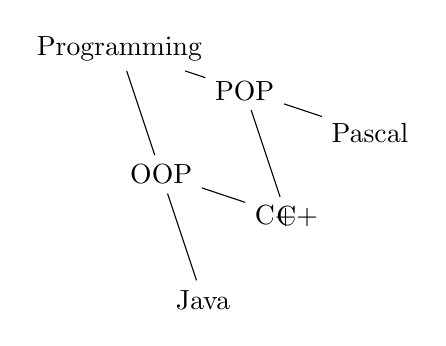
\begin{tikzpicture}[grow=-45]
			\node {Programming}
			child {
				node {OOP}
				child {node {Java}}
				child {node {C++}}
			}
			child {
				node {POP}
				child {node {C}}
				child {node {Pascal}}
			};
		\end{tikzpicture}
	\end{center}
	
\end{document}
